\documentclass[twocolumn,fontsize=11pt]{scrartcl}

% Basic packages
\usepackage[utf8]{inputenc}
\usepackage[T1]{fontenc}
\usepackage{lmodern}
\usepackage[a4paper,margin=1.5cm]{geometry}
\usepackage{multicol}
\usepackage{graphicx}
\usepackage{caption}
\usepackage{subcaption}
\usepackage{amsmath,amssymb}
\usepackage{siunitx}
\usepackage{booktabs}
\usepackage{physics}
\usepackage{float}
\usepackage{hyperref}
\usepackage{physics_macros} % Your custom macros
\usepackage{biblatex} % For bibliography
\addbibresource{bibliography.bib}

% Header and footer
\usepackage{fancyhdr}
\pagestyle{fancy}
\fancyhf{}
\lhead{Star and Stellar Evolution}
\rhead{\thepage}

%Folder
\graphicspath{{plots/}}

% Title
\title{\vspace{-1cm}Stellar Structure Evolution with MESA}
\author{Bruno da Rocha Schultz}
\date{\today}

\begin{document}
\maketitle

\section*{Exercise 1}

\paragraph{Q.1.1:} Why is there only one history file but multiple profile files?

\paragraph{A:} The history file contains the global properties of the star at each time step, while the profile files contain the detailed structure of the star at specific points in time. The history file is updated at each time step, but the profile files are only written at certain intervals. So there is one history file for the entire simulation, but multiple profile files corresponding to different time steps.

\paragraph{Q.1.2:} Show with a plot whether or not the size of the time steps in the history file changes
during the simulation, and discuss why.

\paragraph{A:} The time steps in the history file do change during the simulation. This is because MESA uses an adaptive time-stepping algorithm to ensure that the simulation progresses at a rate that captures the important changes in the star's structure and evolution. The time steps are smaller during rapid changes (like during a shell flash) and larger during more stable phases. Cf. Figure \ref{fig:time_steps} for a plot of the time steps recorded in the history file. 

\begin{figure}[htbp]
    \centering
    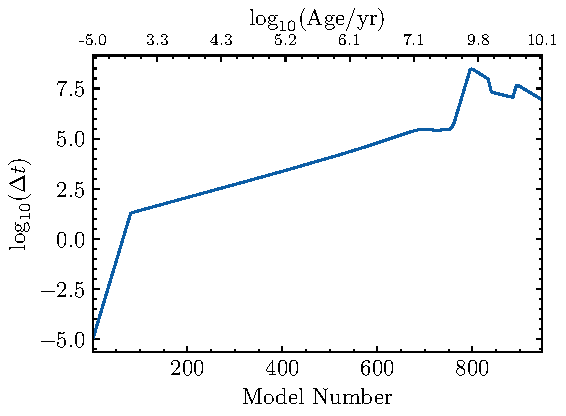
\includegraphics{log_dt_vs_model_number.pdf}
    \caption{Time steps recorded in the history file. The x-axis shows the model number (bottom) and the logarithm of the stellar age (top). The y-axis shows the logarithm of the time step size.}
    \label{fig:time_steps}
\end{figure}

\paragraph{Q.1.3:} Similarly, show with a plot whether or not the grid spacing in a profile file of your
choice is constant, and discuss why. From this plot, also infer which zone is the most  
central zone (zone number 1 or the zone with the highest number).

\paragraph{A:} The grid spacing in a profile file is not constant. MESA uses a non-uniform grid so it can better capture important changes inside the star, making the grid finer where the structure changes quickly and coarser where things are more uniform. In Figure \ref{fig:grid_spacing}, the top graph shows that zone number 1 is at the surface, while the highest zone number is at the center. The bottom graph shows that the spacing between zones (measured as \(\log_{10}(\Delta R / R)\)) is not the same everywhere, confirming that the grid is not evenly spaced. Here, \(\Delta R\) is the difference in radius between adjacent zones, i.e. \(\Delta R = R_{i+1} - R_i\).
%
\begin{figure}[htbp]
    \centering
    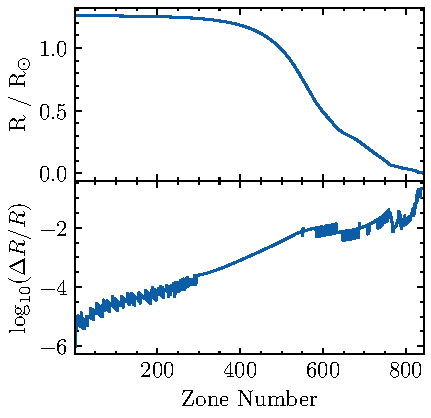
\includegraphics{R_vs_zone.pdf}
    \caption{Grid spacing in a profile file. The x-axis shows the zone number. Top: The radius of each zone.}
    \label{fig:grid_spacing}
\end{figure}
%
\paragraph{Q.1.4:} Which burning stages did the simulation go through, and where did that burning take
place? Graphically Illustrate your answer

\paragraph{A:} Only after the star reaches the zero-age main sequence, defined as the point where the nuclear luminosity exceeds \(99\%\) of the total luminosity (\(\sim 4 \times 10^7\)), is there significant hydrogen burning. Due to the imposed limit \texttt{he\_core\_mass\_limit=0.1}, the star does not reach the conditions necessary for helium burning. 
Figure \ref{fig:q14_luminosity} displays the evolution of hydrogen and helium burning luminosities as the star ages. After the star reaches the ZAMS, hydrogen burning is significant, while helium burning remains negligible for the entire simulation. To indicate where hydrogen burning takes place, Figures \ref{fig:q14_abundancy_H} and\ref{fig:q14_abundancy_e} show the abundances of hydrogen and helium as functions of mass coordinate and stellar age for different late-stage profiles. These plots demonstrate that hydrogen burning is confined to the innermost \(\lesssim 0.15 \text{M}_\odot\)  throughout the simulated period.

\begin{figure}[htbp]
    \centering
    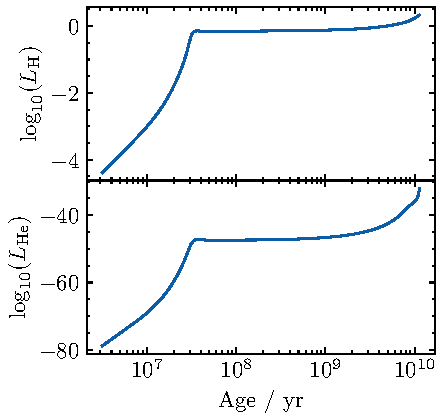
\includegraphics{q14_luminosity.pdf}
    \caption{Hydrogen and helium burning luminosities as a function of stellar age.}
    \label{fig:q14_luminosity}
\end{figure}
\begin{figure}[htbp]
    \centering
    
\includegraphics{q14_abundancy_H.pdf}
    \caption{Hydrogen abundance as a function of mass coordinate and stellar age. The colorbar indicates the hydrogen mass fraction. Hydrogen burning occurs in the core, where the abundance decreases over time.}
    \label{fig:q14_abundancy_H}
\end{figure}
\begin{figure}[htbp]
    \centering
    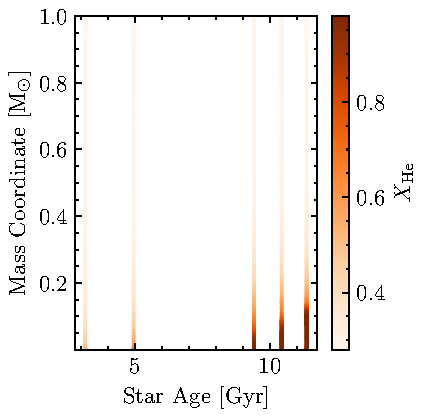
\includegraphics{q14_abundancy_He.pdf}
    \caption{Helium abundance as a function of mass coordinate and stellar age. The colorbar indicates the helium mass fraction. Helium accumulates in the core as hydrogen is fused.}
    \label{fig:q14_abundancy_e}
\end{figure}
\paragraph{Q.1.5:} During the evolution of the stellar model, on what timescales does contraction or expansion occur? You can estimate the contraction/expansion timescale as \(\left|R/\dot{R}\right|\). Show this in a plot with \texttt{model\_number} on the x-axis. Furthermore, show the evolution of the three timescales mentioned above in this plot, and explain in your answer how you defined them. Discuss why the model follows certain timescales during different phases of the simulation.

\paragraph{A:} The contraction or expansion timescale can be estimated as \(\left|R/\dot{R}\right|\), where \(R\) is the radius of the star and \(\dot{R}\) is the time derivative of the radius. This can be calculated from the history file, where the radius and its change over time are recorded. The evolution of the contraction/expansion timescale can be plotted against the model number, showing how the star's size changes over time. We calculate the timescales of stellar evolution as follows:
\begin{align*}
    \tau_{\text{dyn}} &\simeq 0.02 \left(\frac{R}{\Rsun}\right)^{3/2} \left(\frac{\Msun}{M}\right)^{1/2} \text{days}, \\
    \tau_{\text{KH}} &\simeq 1.5 \times 10^7\left(\frac{M}{\Msun}\right)^{2} \frac{\Rsun}{R}\frac{\Lsun}{L} \text{years}, \\
    \tau_{\text{nuc}} &\simeq 1.5 \times 10^6\left(\frac{R}{\Rsun}\right)^{2} \left(\frac{M}{\Msun}\right)^{-1} \text{years}.
\end{align*}
During the pre-main sequence phase, the star contracts under the influence of gravity, leading to a decrease in radius. As the the star contracts, the dynamical timescale (the time it takes for the star to achieve HE\footnote{hydrostatic equilibrium}) also drops, because the star is becoming more compact and can respond more quickly to changes in its internal structure (\(\tau_{\text{dyn}} \propto R^{3/2}\)). Furthermore, the Kelvin-Helmholtz timescale (the time it takes for the star to achieve TE\footnote{thermal equilibrium}) also decreases since . Since during this phase nuclear fusion is not yet active, one can clear see that the evolution of the star occur at the thermal timescale (\(\tau_{\text{KH}} \simeq 10^7 \text{yr}\)).

\section{Exercise 2}

\paragraph{Q2.1:} : In terms of relative mass coordinate (q), what parts of your star are convective at the
terminal-age main sequence (TAMS)? Use information about temperature gradients in
a profile to show this in a plot.

\paragraph{A:} 

\printbibliography

\end{document}
